\documentclass[12pt]{article}
\usepackage{amssymb,amsmath,amsthm,tikz,multirow,graphicx,xcolor,subfigure}
\usetikzlibrary{calc,arrows}

\begin{document}

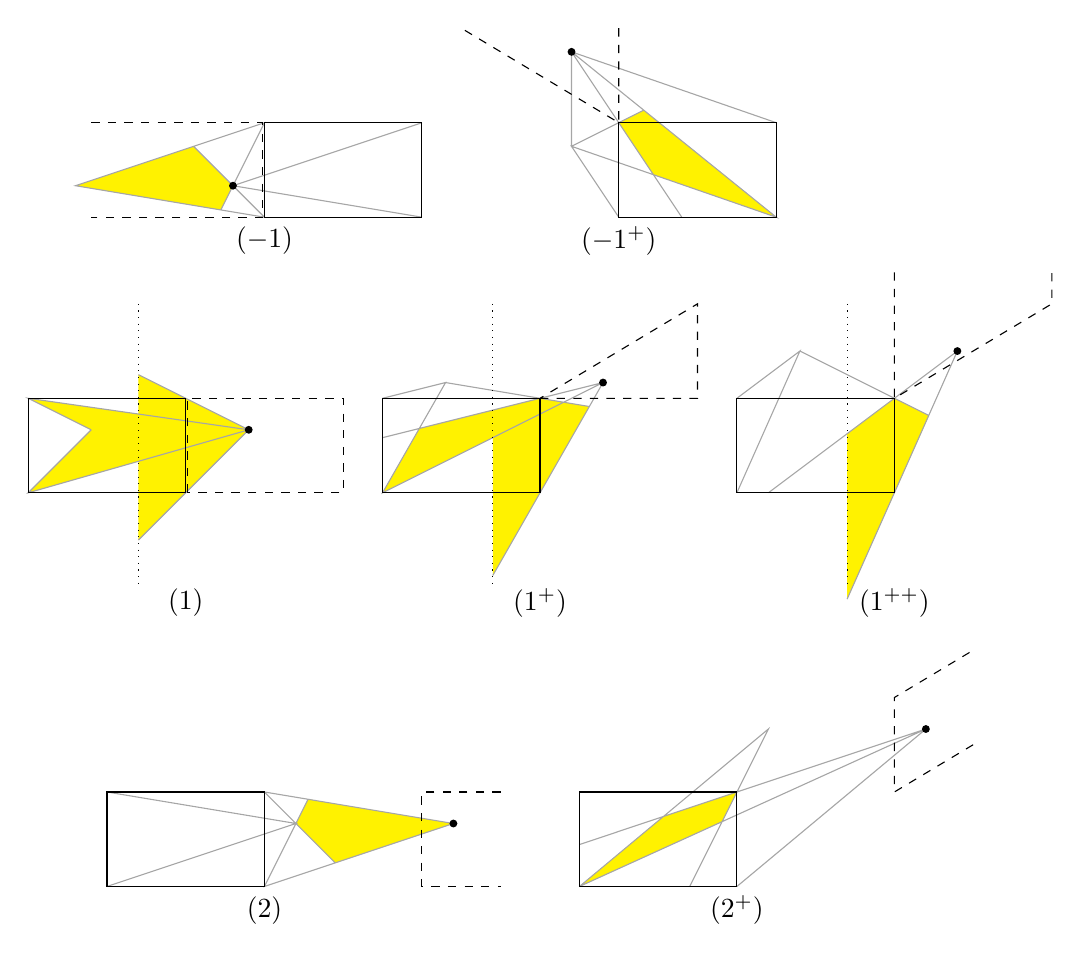
\begin{tikzpicture}[>=latex,scale=1]

%% -1

\begin{scope}[shift={(3cm, 3.5cm)}]


\fill[yellow]
	(-3.4,-0.2) -- (-1.554,-0.508) -- (-1.4,-0.2) -- (-1.9,0.3);

\draw[gray!70]
	(1,-0.6) -- (-1.4,-0.2) -- (1,0.6)
	(-1.9,0.3) -- (-1,-0.6) -- (-3.4,-0.2) -- (-1,0.6) -- (-1.554,-0.508);

\draw
	(-1,-0.6) rectangle (1,0.6);

\draw[dashed]
	(-3.2,0.6) -- (-1.02,0.6) -- (-1.02,-0.6) -- (-3.2,-0.6);
	
\fill (-1.4,-0.2) circle (0.05);

\node at (-1,-0.9) {($-1$)};


\begin{scope}[xshift=4.5cm]

\fill[yellow]
	(-1,0.6) -- (-0.682,0.759) -- (1,-0.6) -- (-0.56,-0.06);

\draw[gray!70]
	(-1,-0.6) -- (-1.6,0.3) -- (1,-0.6) -- (-1.6,1.5) -- (-0.2,-0.6)
	(-0.682,0.759) -- (-1.6,0.3) -- (-1.6,1.5) -- (1,0.6);

\draw
	(-1,-0.6) rectangle (1,0.6);

\draw[dashed]
	(-1,1.8) -- (-1,0.6) -- (-3,1.8) -- (-3,1.8);
	
\fill (-1.6,1.5) circle (0.05);

\node at (-1,-0.9) {($-1^+$)};

\end{scope}


\end{scope}

%% 1


\fill[yellow]
	(-0.2,0.2) -- (-1,0.6) -- (0.4,0.4) -- (0.4,0.9) -- (1.8,0.2)-- (0.4,-1.2) -- (0.4,-0.2) --  (-1,-0.6) -- (-0.2,0.2);

\draw[gray!70]
	(0.4,-1.2) -- (1.8,0.2)--  (0.4,0.9)
	(-0.2,0.2) -- (-1,-0.6) -- (1.8,0.2)--  (-1,0.6) -- (-0.2,0.2);

\draw
	(-1,-0.6) rectangle (1,0.6);

\draw[dashed]
	(1.02,-0.6) rectangle (3,0.6);

\draw[dotted]
	(0.4,1.8) -- (0.4,-1.8);
	
\fill (1.8,0.2) circle (0.05);

\node at (1,-2) {(1)};


\begin{scope}[xshift=4.5cm]

\fill[yellow]
	(-1,-0.6) -- (-0.533,0.217) -- (1,0.6) -- (1.626,0.496) -- (0.4,-1.65) -- (0.4,0.1);

\draw[gray!70]
	(-1,0.6) -- (-0.2,0.8) --  (-1,-0.6) -- (1.8,0.8)
	(-1,0.1) -- (1.8,0.8) --  (0.4,-1.65)
	(-0.2,0.8) -- (1.626,0.496);

\draw
	(-1,-0.6) rectangle (1,0.6);

\draw[dashed]
	 (1,0.6) -- (3,0.6) -- (3,1.8) -- (1,0.6);

\draw[dotted]
	(0.4,1.8) -- (0.4,-1.8);
	
\fill (1.8,0.8) circle (0.05);

\node at (1,-2) {($1^{+}$)};

\end{scope}


\begin{scope}[xshift=9cm]

\fill[yellow]
	(1,0.6) -- (1.44,0.38) -- (0.4,-1.95) -- (0.4,0.15);

\draw[gray!70]
	(-1,0.6)-- (-0.2,1.2) -- (-1,-0.6)
	(-0.6,-0.6) -- (1.8,1.2) --  (0.4,-1.95)
	(-0.2,1.2) -- (1.44,0.38);

\draw
	(-1,-0.6) rectangle (1,0.6);

\draw[dashed]
	(1,2.2) -- (1,0.6) -- (3,1.8) -- (3,2.2);

\draw[dotted]
	(0.4,1.8) -- (0.4,-1.8);
	
\fill (1.8,1.2) circle (0.05);

\node at (1,-2) {($1^{++}$)};

\end{scope}

%% 2

\begin{scope}[shift={(1cm, -5cm)}]

\fill[yellow]
	(3.4,0.2) -- (1.9,-0.3) -- (1.4,0.2) -- (1.554,0.508);

\draw[gray!70]
	(-1,0.6) -- (1.4,0.2) --  (-1,-0.6)
	(1.9,-0.3) -- (1,0.6) -- (3.4,0.2) --  (1,-0.6) -- (1.554,0.508)
	;

\draw
	(-1,-0.6) rectangle (1,0.6);

\draw[dashed]
	(4,0.6) -- (3,0.6) -- (3,-0.6) -- (4,-0.6);
	
\fill (3.4,0.2) circle (0.05);

\node at (1,-0.9) {(2)};


\begin{scope}[xshift=6cm]


\fill[yellow]
	(1,0.6) -- (0.812,0.224) -- (-1,-0.6) -- (0.067,0.289);

\draw[gray!70]
	(-1,-0.6) -- (1.4,1.4) --  (0.4,-0.6)
	(-1,-0.6) -- (3.4,1.4) --  (1,-0.6)
	(3.4,1.4) -- (-1,-0.067);

\draw
	(-1,-0.6) rectangle (1,0.6);

\draw[dashed]
	(4,1.2) -- (3,0.6) -- (3,1.8) -- (4,2.4);
	
\fill (3.4,1.4) circle (0.05);

\node at (1,-0.9) {($2^+$)};

\end{scope}

\end{scope}

\end{tikzpicture}

\end{document}